\section{Agenti Razionali}
Quando si spiega l’attività umana, è spesso utile fare dichiarazioni come le seguenti: \textit{"Janine ha preso l'ombrello perché lei crede che possa piovere"}. Queste affermazioni fanno uso di una \textbf{psicologia popolare} (folks psychology) che fa riferimento al complesso di teorie, credenze e abilità cognitive e comprende la capacità di intuire il funzionamento della mente e di predirne il comportamento.

L'azione \textit{"Janine ha preso l'ombrello"} a seguito della credenza/intuizione \textit{"lei crede che possa piovere"}.

\subsection{Sistema Intenzionale}
Il filosofo Daniel Dennett ha coniato il termine \textbf{sistema intenzionale} per descrivere entità \textit{“Il cui comportamento può essere previsto dal metodo di attribuzione di credenze, di desideri e di acume razionale”}. Quindi secondo questa definizione è opportuno chiedersi se è legittimo o utile attribuire credenze e desideri ai sistemi informatici.
\paragraph{}
L'accademico Jhon McCarthy afferma che ci sono occasioni in cui ascrivere una macchina come sistema intenzionale è appropriata, ad esempio, quando l'iscrizione ci aiuta a capire la struttura della macchina, il suo comportamento passato o futuro, o come ripararla o migliorarla.

Dobbiamo tenere a mente però che più i sistemi di calcolo diventano complessi, più hanno bisogno di astrazioni e metafore potenti per spiegare il loro funzionamento, le spiegazioni di basso livello spesso diventano impraticabili. \textbf{Le nozioni intenzionali sono quindi astrazioni}, che forniscono un modo semplice e familiare per descrivere, spiegare e prevedere il comportamento di sistemi complessi. Quindi qualsiasi sistema, più o meno complesso, può essere definito come sistema intenzionale (e.g. interruttore della luce, Amazon Alexa, robot aspirapolvere, ...) le quali nozioni intenzionali sono tendiamo a vederle come astrazioni, non ci preoccupiamo del loro funzionamento nel dettaglio.

Ma anche importanti sviluppi nella computazione sono basati su astrazioni, basti pensare ai linguaggi di programmazione che ci astraggono dal linguaggio macchina, e anche i concetti di:
\begin{itemize}
    \item Oggetti
    \item Procedure/funzioni
    \item Tipi di dati
\end{itemize}

Gli agenti intelligenti e, in particolare, i sistemi intenzionali, rappresentano un ulteriore (e
potente) astrazione.

\subsection{Practical Reasoning (Ragionamento su Azioni)}
Il practical reasoning è il ragionamento sulle azioni, sul processo di capire cosa fare, l'uso della ragione per decidere come agire. Il practical reasoning si distingue dal Theoretical Reasoning, che riguarda solo le credenze non le azioni. 

Il Practical Reasoning è caratterizzato da due attività:
\begin{itemize}
    \item Deliberazione: Quale stato di cose vogliamo raggiungere (l'output sono le \textbf{intenzioni}).
    \item Pianificazione o means-ends reasoning: Come possiamo raggiungere gli obiettivi (l'output è il soddisfacimento delle intenzioni, raggiungere lo stato di cose).
\end{itemize}

Deliberazione e means-ends reasoning sono processi computazionali, come tali in tutti gli agenti reali questi processi avranno risorse limitate (e.g. il tempo, lo spazio, ...). Quindi il calcolo è una risorsa preziosa per gli agenti perché serve per controllare il suo ragionamento ed è importante che non agiscano a tempo indeterminato, perché anche il tempo è una risorsa.
\textbf{Con intenzioni ci riferiamo allo stato di cose che un agente ha scelto di raggiungere}.

\subsection{Proattività e Intenzioni}
Anche se un agente è un sistema informatico è intelligente, non perché ha consapevolezza o capacità extra-programma, ma se riusciamo ad attribuirgli alcune caratteristiche, tra cui, la \textbf{proattività}. 
Il ruolo delle intenzioni è quello di favorire la proattività, cioè tendono portare ad agire, all’azione.
\begin{center}
    \includegraphics[scale=0.5]{images/agente_e_proattività.png}
\end{center}

Il filosofo Brattman osserva che le intenzioni giocano un ruolo molto più forte nell’influenzare l’azione rispetto ad altri atteggiamenti proattivi come il desiderio. Infatti \textbf{le intenzioni non possono essere in contrasto, mentre invece i desideri si}.

Quindi possiamo dire che le intenzioni hanno le seguenti proprietà:
\begin{itemize}
    \item \textbf{Problemi}: Le intenzioni pongono problemi agli agenti, se ho un intenzione \begin{math} \varphi \Rightarrow alloco\;risorse : \exists piano \; per\;eseguire\;\varphi \end{math}
    \item \textbf{Le intenzioni vincolano il futuro practical reasoning}, quindi non posso generare intenzioni che vanno in conflitto tra loro: Se ho il desiderio di andare in piscina ma devo andare a lavoro, la piscina rimane un desiderio, il lavoro l'intenzione.
    \item \textbf{Persistenza}: Gli agenti monitorano il successo delle loro intenzioni e sono inclini a riprovare se i loro tentativi falliscono, solo se la motivazione dell’intenzione non sussiste più, è razionale abbandonare tale intenzione.
    \item Gli agenti credono che le loro intenzioni siano possibili. Se voglio andare in piscina credo che la piscina sia aperta e che io posso fare la mia attività.
    \item Gli agenti non credono che non porteranno avanti le loro intenzioni.
    \item In determinate circostanze, gli agenti credono che realizzeranno le loro intenzioni..
    \item \textbf{Effetti collaterali}: Gli agenti non devono necessariamente avere intenzione su tutti gli effetti.
collaterali delle loro intenzioni (e.g. ho una carie, affronto il dolore per curarla).
\end{itemize}

\section{Realizzazione di Agenti che Sfruttano il Practical Reasoning}

\subsection{Agent Control Loop Version 1}

\begin{tcblisting}{breakable,listing only, listing options={language=Python,aboveskip=0pt,belowskip=0pt}, size=fbox}
while true do:
    # deliberazione
    observe the world;
    update internal world model;
    deliberate about what intention to achieve next;
    
    # pianificazione
    use means-ends reasoning to get a plan;
    execute the plan;
\end{tcblisting}

I processi di deliberazione e means-ends reasoning non sono istantanei, hanno un costo in termini di tempo, questo significa che quando ottengo un piano potrebbe non essere più quello che mi serve. Osservando questa timeline possiamo fare alcune deduzioni:

\begin{center}
    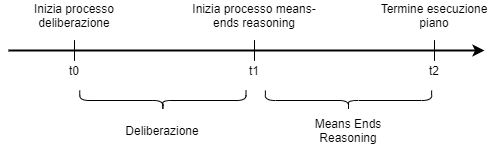
\includegraphics[scale=0.6]{images/deliberazion_meansend_timechart.png}
\end{center}

Definiamo come tempo per deliberare:
\begin{displaymath}
    T_{deliberazione} = t_1 - t_0
\end{displaymath}
\begin{displaymath}
    T_{means-ends-reasoning} = t_2 - t_1
\end{displaymath}

La \textbf{deliberazione è ottimale} se al tempo $t_1$, l’agente ha selezionato l’intenzione da raggiungere che sarebbe stata ottimale se fosse stata raggiunta all’istante $t_0$. A meno che il tempo $T_{deliberazione}$ sia estremamente piccolo, l’agente corre il rischio che l’intenzione selezionata non sia pi`u ottimale nel momento in cui l’agente l’ha deliberata. Ma la fase di deliberazione è solo metà del problema: l’agente deve ancora determinare come realizzare l’intenzione. 

Quindi, \textbf{l’agente avrà un comportamento complessivo ottimale} nelle seguenti circostanze:
\begin{itemize}
    \item $T_{deliberazione} \rightarrow 0$: Quando il tempo impiegato per i processi di deliberazione e di means-ends reasoning è incredibilmente piccolo.
    \item Quando l'ambiente è garantito rimanere statico mentre l’agente sta eseguendo i processi di deliberazione e di means-ends reasoning.
    \item Quando un’intenzione ottimale se raggiunta al tempo $t_0$ (momento in cui si osserva l'ambiente) è garantita rimanere ottimale fino al tempo $t_2$ (momento in cui l’agente ha determinato le azioni per raggiungere l’intenzione).
\end{itemize}

\subsection{Agent Control Loop Version 2}
\begin{tcblisting}{breakable, listing only, listing options={language=Python, aboveskip=0pt, belowskip=0pt, escapechar=*}, size=fbox}
# initial beliefs B := B0;
while true do
    get next percept *$\rho$*;
    B := brf(B, *$\rho$*);
    I := deliberate(B);
    *$\pi$* := plan(B, I);
    execute(*$\pi$*)
\end{tcblisting}

Analizziamo lo pseudo codice soprastante con particolare attenzione alla funzione \textbf{brf}, che sta per Belief Revision Function, ovvero la funzione che si occupa della revisione delle credenze:
\begin{itemize}
    \item \textit{get next percept $\rho$;} registriamo le credenze rilevati in qualche modo (e.g. tramite l'utilizzo di sensori).
    \item \textit{B := brf(B, *$\rho$*);} Aggiorna i beliefs B sulla base di quelli correnti e delle credenze (non monotona perché devo rivedere le mie credenze o eliminarne qualcuna).
    \item \textit{I := deliberate(B);} deliberiamo le intenzioni basate sulla credenze aggiornate.
    \item \textit{$\pi$ := plan(B, I);} pianificazione di un piano $\pi$.
    \item \textit{execute($\pi$)} esegue i piani.
\end{itemize}

\subsection{BDI: Belief Desire Intention}
\subsubsection{Agent Control Loop Version 3}
\textbf{Belief Desire Intention (BDI)} è un tipo di architettura per agenti, applicata nella seguente implementazione, che inizia cercando di capire quali sono le opzioni a sua disposizione (desires) sulla base delle proprie informazioni e credenze (beliefs), in ultimo sceglie tra le opzioni possibili e definisce delle intenzioni (intentions).

\begin{tcblisting}{breakable, listing only, listing options={language=Python, aboveskip=0pt, belowskip=0pt, escapechar=*}, size=fbox}
B := *$B_0$*;
I := *$I_0$*;
while true do
    get next percept *$\rho$*;
    B := brf(B, *$\rho$*);
    D := options(B, I);
    I := filter(B, D, I);
    *$\pi$* := plan(B, I);
    execute(*$\pi$*)
\end{tcblisting}

A differenza della versione precedente (v2) dovremmo definire dei desires D basandoci su B e I. Inoltre assumiamo che a $t_0$ di avere beliefs B e intentions I definite.
Analizziamo le novità rispetto al codice precedente:
\begin{itemize}
    \item \textit{D := options(B, I);} l'agente genera un insieme di possibili alternative, desideri D.
    \item \textit{I := filter(B, D, I);} Quando un'opzione è restituita da \textbf{flter} e quindi è scelta dall'agente come intenzione I, diciamo che l'agente ha fatto un \textbf{commitment}, ovvero ha preso un impegno, verso tale opzione. 
\end{itemize}

Il \textbf{commitment} implica \textbf{persistenza temporale}, un'intenzione, una volta adottata, non dovrebbe immediatamente essere abbandonata. Quindi viene automatico chiedersi quanto a lungo un intenzione dovrebbe persistere? Il meccanismo che una agente usa per determinare quando e come un'intenzione possa essere abbandonata è conosciuta come \textbf{commitment strategies}.
Sono state identificate tre principali strategie:
\begin{enumerate}
    \item \textbf{Blind Commitment (Fanatico)}: Un agent blind committed continuerà a mantenere un'intenzione fino a quando non crederà che l'intenzione sia stata effettivamente raggiunta. Il blind commitment è talvolta indicato anche come fanatical commitment.
    \item \textbf{Open-Minded Commitment}: Un agente open-minded committed manterrà un'intenzione fintanto che la ritiene, la crede possibile.
    \item \textbf{Single-Minded Commitment (Risoluto)}: Un agente single-minded committed continuerà a mantenere un'intenzione perché non ritiene che l'intenzione sia stata raggiunta, o che non sia più possibile raggiungerla.
\end{enumerate}

Agent Control Loop Version 3 è un agente \textbf{overcommited}, cioè impegnato in modo eccessivo ad ultimare le sue intenzioni, questo perché il piano $\pi$ potrebbe richiedere troppo tempo senza considerare i cambiamenti esterni.

\subsubsection{Agent Control Loop Version 4: Ripianificazione}
La ripianificazione, nel caso in cui qualcosa vada storto o se le intenzioni I non sono più corrette, riduce il commitment dell'agente.
Introduciamo la funzione \textbf{sound} che simula i passi di un piano e verifica che siano ancora corrette. Questa funzione ha costo lineare a differenza della \textit{plan} che è più complessa.

\begin{tcblisting}{breakable, listing only, listing options={language=Python, aboveskip=0pt, belowskip=0pt, escapechar=*}, size=fbox}
B := *$B_0$*;
I := *$I_0$*;
while true do
    get next percept *$\rho$*;
    B := brf(B, *$\rho$*);
    D := options(B, I);
    I := filter(B, D, I);
    *$\pi$* := plan(B, I);
    
    while not empty(*$\pi$*) do
        # head(*$\pi$*) restituisce la prima azione del piano 
        *$\alpha$* := head(*$\pi$*);
        execute(*$\alpha$*);
        
        # nuovo piano: le restanti azioni (la coda)
        *$\pi$* := tail(*$\pi$*);
        get next percept *$\rho$*;
        B := brf (B, *$\rho$*);
        if not sound(*$\pi$*, I , B) then
            *$\pi$* := plan(B, I )
\end{tcblisting}

L'agente è ancora \textbf{overcommited} rispetto le intenzioni: non si ferma mai valutare se le sue intenzioni siano o meno adeguate.

\subsection{Riconsiderare le Intenzioni}
\subsubsection{Agent Control Loop Version 5}
Per ridurre ulteriormente il commitment modifichiamo l'agente della versione 4 per far si che si fermi a determinare se le intenzioni hanno avuto successo o se sono diventate impossibili da soddisfare (single-minded commitment). Quindi l'agente può \textbf{riconsiderare le sue intenzioni I} ogni volta che il controllo ci dice che:
\begin{itemize}
    \item \textbf{not empty($\pi$)}: Ci sono azioni nel piano.
    \item \textbf{succeeded(I , B)}: Ritiene raggiunte con successo le sue attuali intenzioni.
    \item \textbf{impossible(I , B)}: Crede che le sue attuali intenzioni non siano più possibili.
\end{itemize}

\begin{tcblisting}{breakable, listing only, listing options={language=Python, aboveskip=0pt, belowskip=0pt, escapechar=*}, size=fbox}
B := *$B_0$*;
I := *$I_0$*;
while true do
    get next percept *$\rho$*;
    B := brf(B, *$\rho$*);
    D := options(B, I);
    I := filter(B, D, I);
    *$\pi$* := plan(B, I);
    
    while not empty(*$\pi$*) or
         succeeded(I , B) or
         impossible(I , B) do
        # head(*$\pi$*) restituisce la prima azione del piano 
        *$\alpha$* := head(*$\pi$*);
        execute(*$\alpha$*);
        
        # nuovo piano: le restanti azioni (la coda)
        *$\pi$* := tail(*$\pi$*);
        get next percept *$\rho$*;
        B := brf (B, *$\rho$*);
        if not sound(*$\pi$*, I , B) then
            *$\pi$* := plan(B, I)
\end{tcblisting}

\newpage

\subsubsection{Agent Control Loop Version 6}
Possiamo migliorare la versione precedente facendogli riconsiderare le intenzioni I dopo l'esecuzione di ogni azione del piano.

\begin{tcblisting}{breakable, listing only, listing options={language=Python, aboveskip=0pt, belowskip=0pt, escapechar=*}, size=fbox}
B := *$B_0$*;
I := *$I_0$*;
while true do
    get next percept *$\rho$*;
    B := brf(B, *$\rho$*);
    D := options(B, I);
    I := filter(B, D, I);
    *$\pi$* := plan(B, I);
    
    while not empty(*$\pi$*) or
         succeeded(I , B) or
         impossible(I , B) do
        # head(*$\pi$*) restituisce la prima azione del piano 
        *$\alpha$* := head(*$\pi$*);
        execute(*$\alpha$*);
        
        # nuovo piano: le restanti azioni (la coda)
        *$\pi$* := tail(*$\pi$*);
        get next percept *$\rho$*;
        B := brf (B, *$\rho$*);
        D := options(B, I);
        I := filter(B, D, I);
        
        if not sound(*$\pi$*, I , B) then
            *$\pi$* := plan(B, I)
\end{tcblisting}

C'è da sottolineare il fatto che riconsiderare delle intenzioni costa? Un agente che non si ferma per riconsiderare le proprie intenzioni abbastanza spesso continuerà a tentare di raggiungere le sue intenzioni anche se sono impossibili da raggiungere, d'altro canto un agente che riconsidera costantemente le sue intenzioni potrebbe dedicare un tempo insufficiente a raggiungerle effettivamente.

\subsubsection{Agent Control Loop Version 7}
In questa implementazione incorporiamo una esplicita componente di controllo di meta-livello che decide se eseguire o meno la riconsiderazione, il metodo \textbf{reconsider}. Recondider è una componente di controllo che decide sulla base di un euristica (insieme di strategie, tecniche e procedimenti) che dipende dal dominio.

\begin{tcblisting}{breakable, listing only, listing options={language=Python, aboveskip=0pt, belowskip=0pt, escapechar=*}, size=fbox}
B := *$B_0$*;
I := *$I_0$*;
while true do
    get next percept *$\rho$*;
    B := brf(B, *$\rho$*);
    D := options(B, I);
    I := filter(B, D, I);
    *$\pi$* := plan(B, I);
    
    while not empty(*$\pi$*) or
         succeeded(I , B) or
         impossible(I , B) do
        # head(*$\pi$*) restituisce la prima azione del piano 
        *$\alpha$* := head(*$\pi$*);
        execute(*$\alpha$*);
        
        # nuovo piano: le restanti azioni (la coda)
        *$\pi$* := tail(*$\pi$*);
        get next percept *$\rho$*;
        B := brf (B, *$\rho$*);
        if reconsider(I , B) then
            D := options(B, I);
            I := filter(B, D, I);
        
        if not sound(*$\pi$*, I , B) then
            *$\pi$* := plan(B, I)
\end{tcblisting}

\subsubsection{Possibili interazioni}
Le possibili interazioni la componente di controllo di meta-livello, ovvero la funzione \textit{reconsider}, e deliberazione sono:

\begin{center}
    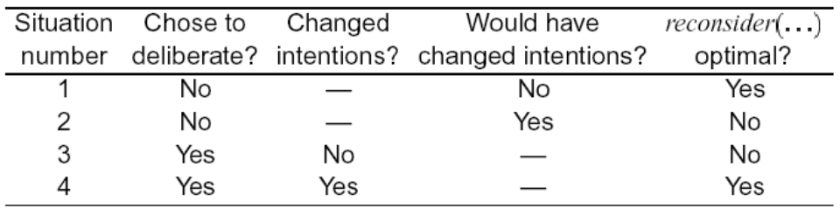
\includegraphics[scale=0.4]{images/Riconsidera Intenzioni Casi D'uso.png}
\end{center}

\begin{enumerate}
    \item L’agente non ha scelto di deliberare, e come conseguenza, non ha scelto di cambiare le intenzioni, se avesse scelto di deliberare, non avrebbe cambiato le intenzioni. In questa situazione, la funzione \textit{reconsider} si sta comportando in modo ottimale perché mi risponde di non deliberare.
    \item L’agente non ha scelto di deliberare, ma se lo avesse fatto avrebbe cambiato le intenzioni. In questa situazione, la funzione \textit{reconsider} non si sta comportando in modo ottimale.
    \item L’agente ha scelto di deliberare, ma non ha cambiato intenzioni. In questa situazione, la funzione reconsider non si comporta in modo ottimale.
    \item L’agente ha scelto di deliberare e ha cambiato intenzioni. In questa situazione, la funzione reconsider si sta comportando in modo ottimale.
\end{enumerate}

Quindi il comportamento della funzione \textit{reconsider} dipende da quanto cambia l'ambiente che porta ad un cambio delle intenzioni.

\subsubsection{Riconsiderazione ottimale delle intenzioni}
Kinny e Georgeff investigano in maniera sperimentale l’efficacia delle strategie, nello specifico su due diversi tipi di strategia di riconsiderazione sono stati utilizzati:
\begin{itemize}
    \item \textbf{Bold agents (audaci)} agenti che non si fermano mai a riconsiderare le intenzioni.
    \item \textbf{Cautious agents (cauti)} si ferma a riconsiderare le intenzioni dopo ogni azione.
\end{itemize}

Possiamo definire $\gamma$ come il grado di dinamismo dell’ambiente dove, se $\gamma$ è basso l’ambiente non cambia rapidamente invece se $\gamma$ è alto l'ambiente cambia rapidamente:
\begin{itemize}
    \item \textbf{$\gamma$ alto, ambiente dinamico}: Gli agenti audaci preformano meglio perché quelli cauti perdono tempo a riconsiderare i propri impegni mentre agenti audaci sono impegnati a lavorare per raggiungere le loro intenzioni.
    \item \textbf{$\gamma$ basso, ambiente statico}: Gli agenti cauti tendono a preformare meglio perché sono in grado di riconoscere quando le intenzioni non sono più corrette, traendo anche vantaggio da situazioni fortuite e nuove opportunità quando si presentano.
\end{itemize}

\newpage

\subsection{PRS: Procedural Reasoning System}
PRS, che sta per Procedural Reasoning System, fu la prima architettura per agenti sviluppata ad includere il paradigma BDI (Belief, Desire, Intention) ed ha diverse applicazioni, come ad esempio il sistema di controllo del traffico aereo all'aereoporto di Sydney.

L'Architettura può essere rappresentata come segue:
\begin{center}
    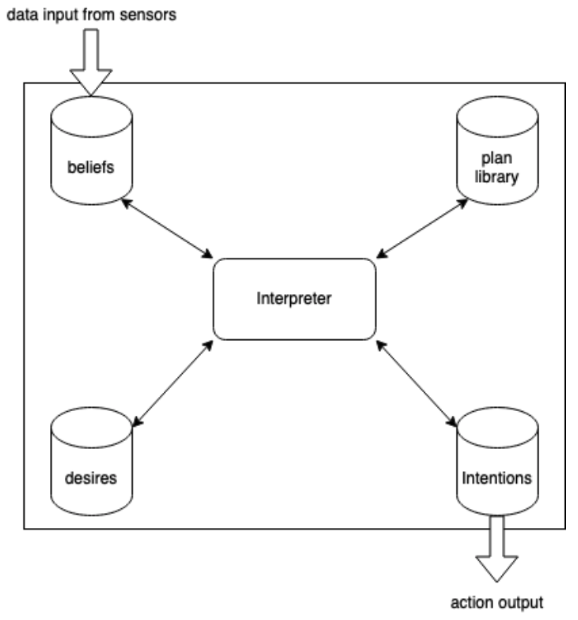
\includegraphics[scale=0.4]{images/PRS.png}
\end{center}
E' un interprete che utilizza una librerie di piani precompilati e un insieme di desideri in combinazione con dei belief per determinare delle azioni basate su intenzioni.

Ponendo l'attenzione sulla \textbf{libreria di piani} possiamo pensare al comportamento di un semplice programma che, con i suoi blocchi condizionali, va a identificare specifici comportamenti da attuare durante la sua esecuzione e si comporta come un \textit{pianificatore}, maggiori sono i blocchi condizionali più saranno i casi d'uso che il programma riuscirà a gestire. 
Le architetture PRS anziché utilizzare un pianificatore utilizza una libreria di piani che sono precompilati dai programmatori, che sono costituiti da:
\begin{itemize}
    \item \textbf{Goal}: Post condizione del piano.
    \item \textbf{Contesto}: Precondizione del piano (prerequisiti).
    \item \textbf{Corpo}: Sequenza di azioni
\end{itemize}
Quindi \textbf{il piano viene scelto dall'interprete nella libreria sulla base del Goal e del Contesto}. Ma in PRS i piani possono essere più complessi, in particolare possono contenere a loro volta altri Goal.
Quindi un agente PRS ha un insieme di piani, alcuni belief iniziali riguardo l'ambiente (e.g. rappresentati come fatti Prolog) e un goal iniziale.